% =====================================================================
%  §6. Лестница моделей и цена усложнения
%
%  ЖАНР (STYLE.md): учебная литература. Ни путей, ни имён программ, ни
%  номеров гипотез. Прослеживаемость — ключи \srckey{6.x} и приложение.
%
%  Содержательная основа: BRIEF_FOR_D_teaching_ladder.md §7; SYNTHESIS.md
%  §4, §7.1-7.3; опирается на теорему о выровненном анализаторе (§1).
% =====================================================================
\section{Лестница моделей и цена усложнения}
\label{sec:ladder}
\markboth{§\thesection. Лестница моделей}{}

К этому месту курс собрал целый набор возможных усложнений модели: конечная проводимость и
степенное рассеяние (§3), явное просачивание с собственной фазой (§1), комплексный перекрёстный
член, второй реальный элемент тракта вместо идеального анализатора (§1). Возникает практический
вопрос: в каком порядке их вводить, и как узнать, что усложнение того стоило? В этом параграфе
собран весь путь~--- от исходной геометрической модели §2 до модели, на которую опирается
дальнейшая часть курса,~--- и явно показана \term{цена} каждой ступени.

\begin{tcolorbox}[enhanced,colback=cPanel,colframe=cGrid,boxrule=0.8pt,arc=2pt,
                  title={\bfseries\color{cAccent} Пререквизиты},coltitle=cAccent,
                  attach boxed title to top left={xshift=6pt,yshift=-2pt},
                  boxed title style={colback=cPanel,boxrule=0pt,arc=0pt},top=10pt]
\textbf{Нужно знать:} §2 (геометрическая модель), §3 (Друде, степенные потери), §1 (просачивание,
теорема о выровненном анализаторе); понятие информационного критерия хотя бы на уровне «больше
параметров даёт лучший $\chi^2$ почти всегда, поэтому сравнивать модели по одному $\chi^2$
нечестно» (формальный вывод $\AIC=-2\ln L+2k$~--- в §8).\\[0.3em]
\textbf{Знать НЕ нужно:} вывод формулы AIC~--- в этом параграфе она используется как готовый
инструмент сравнения, обоснование появится в §8.
\end{tcolorbox}

% ---------------------------------------------------------------------
\subsection{Принцип: усложнение должно быть оплачено}
\label{subsec:pay-principle}

\begin{intuition}
Добавление любого нового свободного параметра почти никогда не ухудшает $\chi^2$ на тех же
данных, на которых модель обучена,~--- в худшем случае оптимизатор просто не воспользуется новой
свободой. Значит, сравнение моделей \emph{по одному лишь} $\chi^2$ всегда выберет более сложную
модель, даже если новый параметр не отражает никакой реальной физики. Нужна валюта, в которой
усложнение \emph{стоит} чего-то,~--- и такая валюта, штрафующая за каждый дополнительный
параметр,~--- информационный критерий Акаике.
\end{intuition}

\noindent
Практическое правило, которым пользуется этот параграф (полная шкала~--- в §8): изменение
$\dAIC$ порядка единиц означает «не различить»; порядка десятков~--- «уверенное улучшение»;
порядка тысяч~--- «прежняя модель категорически не годится».

% ---------------------------------------------------------------------
\subsection{Лестница для одного элемента тракта}
\label{subsec:ladder-single}

\begin{center}
\footnotesize
\setlength{\tabcolsep}{6pt}
\begin{tabular}{@{}p{0.14\linewidth}p{0.40\linewidth}p{0.40\linewidth}@{}}
\toprule
\textbf{Ступень} & \textbf{Что добавлено} & \textbf{Чем оплачено} \\
\midrule
базовая & чистая геометрическая модель §2 & точка отсчёта \\
$+$ материал & конечная проводимость (Друде) $+$ степенные потери §3 &
$\dAIC\approx-957$ (плотная решётка), $-266$ (разреженный образец)~--- уверенное улучшение на
обоих \\
$+$ свободный диаметр & $\Deff$ отпущен свободно, просачивание ещё не включено & здесь
возникает та самая загадка $\Deff/\Dphys$ из §\ref{sec:electrodynamics} \\
$+$ пин к физическому $D$, без просачивания & $\Deff$ приколочен к измеренному под микроскопом
диаметру & $\dAIC\approx+6167$~--- катастрофа: модель категорически хуже \\
$+$ явное просачивание & $\Deff$ приколочен к эффективному значению, добавлена
частотно-зависимая утечка $\eta(\nu)e^{\jj(\delta_0+2\pi\nu\tleak)}$ (§1) & \textbf{опорная
модель курса}: смещение в глубокой тени $3{,}38\to1{,}25$~дБ, среднеквадратичная ошибка
$2{,}21\to1{,}58$ \\
$+$ перекрёстный член & комплексная, не зависящая от угла добавка $\varepsilon_{\rm cross}$ &
улучшает $\AIC$, но не выдерживает проверку на нескольких образцах одновременно (ниже) \\
\bottomrule
\end{tabular}
\end{center}
\srckey{6.1}

\begin{warning}[: пин к физическому диаметру — не мелкая деталь, а диагностика]
Ступень «пин к физическому $D$» не улучшает модель, а \emph{ломает} её на $\dAIC$ порядка
тысяч~--- переоценивая тень на $7$--$10$~дБ. Это не значит, что физический диаметр измерен
неверно: это значит, что модель, в которую он подставлен, ещё не содержит канала, необходимого
для описания данных при физическом размере провода. Именно эта катастрофа~--- главный
экспериментальный аргумент за существование недостающего физического механизма, который
эффективный диаметр в предыдущих параграфах компенсировал сам (§\ref{sec:electrodynamics}).
\end{warning}

\begin{example}[: катастрофа воспроизводится не на одном образце]\srckey{6.2}
Провал пина к физическому диаметру без просачивания~--- не случайность одного набора измерений:
на трёх независимо измеренных образцах $\dAIC$ от такого пина составляет от нескольких тысяч до
$+9063$ на образце средней плотности. Универсальность провала~--- сильный довод в пользу того, что
недостающий канал общий для всех образцов, а не артефакт одной серии измерений.
\end{example}

% ---------------------------------------------------------------------
\begin{figure}[t]
  \centering
  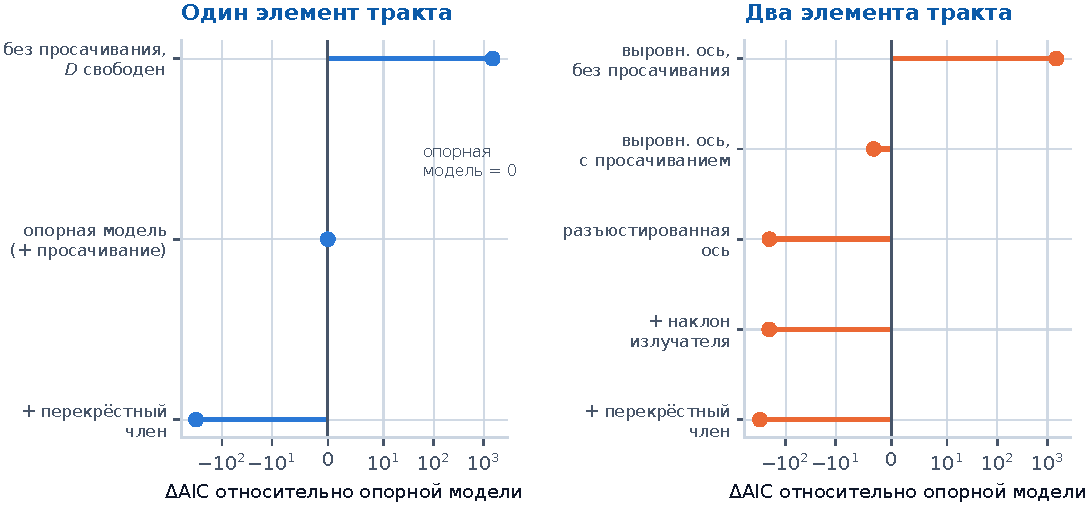
\includegraphics[width=\linewidth]{figures/fig06_ladder.pdf}
  \caption{Ступени лестницы для плотной решётки ($D/P=0{,}71$), информационный критерий
  относительно опорной модели курса. Слева~--- одиночный элемент тракта: от свободного диаметра
  без просачивания (наравне с его точным двух-элементным аналогом при выровненной оси, разница
  $0{,}15$~--- ключ~1.3) до опорной модели и её усложнения перекрёстным членом. Справа~--- та же
  лестница для двух реальных элементов тракта (§\ref{subsec:two-wgp}): пока ось выровнена,
  усложнение до второго реального элемента почти ничего не меняет; выигрыш появляется только
  вместе с разъюстировкой оси, которую отдельно обсуждает предупреждение
  §\ref{subsec:two-wgp}.}
  \label{fig:ladder}
\end{figure}

% ---------------------------------------------------------------------
\subsection{Перекрёстный член: улучшает подгонку, не проходит проверку}
\label{subsec:eps-cross}

Комплексный член $\varepsilon_{\rm cross}$, не зависящий от угла, улучшает согласие с данными на
отдельно взятом образце. Прежде чем принять его как физический эффект, естественно спросить:
одна ли это и та же константа тракта на разных образцах, или же подгонка каждый раз находит
удобное число под конкретный набор данных?

\begin{example}[: проверка на нескольких образцах отвергает гипотезу о константе тракта]\srckey{6.3}
Проверка однородности значения $\varepsilon_{\rm cross}$ между образцами отвергает гипотезу о
единой константе тракта: статистика проверки на однородность равна $761{,}6$ при $10$ степенях
свободы ($p=3{,}8\times10^{-157}$)~--- несовместимо со случайным разбросом вокруг одного истинного
значения. Отдельно, оценки просачивания образца и перекрёстного члена коррелируют между собой на
уровне $0{,}73$ (§1, ключ~1.2)~--- то есть параметр отчасти забирает на себя то, что должно было
бы принадлежать просачиванию.
\end{example}

\begin{intuition}[: как читать этот результат]
Улучшение $\AIC$ на одном образце говорит: «добавленный параметр помогает описать именно эти
данные». Проверка на нескольких образцах говорит нечто другое и более сильное: «помогает ли он
одним и тем же числом, как и должна вести себя константа тракта». Первое~--- необходимое условие
для физической интерпретации параметра, но не достаточное. Перекрёстный член проходит первую
проверку и не проходит вторую~--- значит, улучшение реально, а предложенная физическая
интерпретация (константа приёмного тракта) конкретно для этого параметра~--- нет.
\end{intuition}

% ---------------------------------------------------------------------
\subsection{Два элемента тракта: усложнение, которое не понадобилось}
\label{subsec:two-wgp}

Основная модель курса считает второй элемент тракта (анализатор перед приёмником) идеальным. Но
он~--- такой же реальный элемент, как исследуемый образец, со своим собственным просачиванием.
Соблазн очевиден: заменить идеальный анализатор его полной, реальной моделью и посмотреть, что
скажет подгонка. Это ровно та ситуация, для которой в §1 была доказана \term{теорема о
выровненном анализаторе}: если ось пропускания второго элемента совпадает с осью чувствительности
приёмника, его неидеальность \emph{ненаблюдаема}~--- она сводится к общему множителю, не
зависящему от угла.

\begin{strict}[: предсказание и его проверка (напоминание §1)]
Теорема предсказывает: явное включение второго реального элемента в модель не улучшит согласия
с данными и не сдвинет оценку эффективного диаметра. Измерено: изменение информационного критерия
$\dAIC=+0{,}15$ (усложнённая модель не лучше исходной~--- различие на два порядка меньше даже
самого скромного уверенного улучшения по шкале §\ref{subsec:pay-principle}), оценка эффективного
диаметра совпадает в четырёх значащих цифрах до и после усложнения.
\end{strict}

\begin{intuition}[: почему это ценный педагогический пример]
Модель усложнили честно~--- не отказались от идеи из осторожности, а реализовали её и запустили
подгонку,~--- и она отказалась усложняться ровно так, как было предсказано аналитически \emph{до}
расчёта. Отрицательный результат, полученный дважды (на бумаге и на данных),~--- такой же
полноценный научный результат, как и положительный: он экономит время, которое иначе ушло бы на
интерпретацию шума как физического эффекта.
\end{intuition}

\begin{warning}[: условие теоремы существенно, и с ним связана отдельная лестница]
Если ось второго элемента \emph{разъюстирована} относительно приёмника, условие теоремы
нарушается, и его неидеальность становится наблюдаемой. На данных это заметно: варианты модели,
явно учитывающие разъюстировку оси (и, отдельно, наклон излучателя), дают уверенное улучшение
$\AIC$ по сравнению с версией без такого учёта. Это не противоречит теореме~--- это именно то,
что она предсказывает при нарушении её условия,~--- но означает, что \emph{юстировка} тракта
имеет прямую количественную цену в качестве подгонки, тогда как \emph{полнота} модели анализатора
при аккуратной юстировке цены не имеет.
\end{warning}

% ---------------------------------------------------------------------
\subsection{Типичные ошибки этого параграфа}

\begin{enumerate}[leftmargin=1.6em,itemsep=0.25em]
  \item Сравнивать усложнённую и базовую модель по $\chi^2$ без штрафа за число параметров. Более
        сложная модель почти всегда даст $\chi^2$ не хуже~--- вопрос в том, оправдан ли выигрыш
        (§\ref{subsec:pay-principle}).
  \item Интерпретировать катастрофический $\dAIC$ пина к физическому диаметру как ошибку
        измерения диаметра. Это диагностика недостающего канала модели, а не претензия к
        микроскопии.
  \item Принять улучшение $\AIC$ на одном образце за доказательство физического смысла нового
        параметра. Нужна проверка на нескольких независимых образцах
        (§\ref{subsec:eps-cross})~--- она есть не всегда, и без неё вывод неполон.
  \item Усложнять модель «на всякий случай», не проверив заранее аналитически, не сводится ли
        усложнение к ненаблюдаемому множителю (§\ref{subsec:two-wgp}, теорема §1). Такая проверка
        стоит бумаги и карандаша и экономит недели вычислений.
  \item Спутать «юстировка не имеет значения» с «полнота модели анализатора не имеет значения».
        Верно второе при выполненном условии теоремы; первое неверно всегда.
\end{enumerate}

\clearpage
